\begin{paper}{1}
\begin{header}
\title{Perturbation energy and exchange in the many-body problem.}
\author{W. Heitler}
\location{G\"ottingen}
\note{Received on October 12th 1927.}
\makeheader
\end{header}

\newcommand{\Aikp}[3]{\left({#1}_{#2}^{#3 \vphantom{P_{n!}}}\right)}

\begin{abstract}
Group theory permits, without essentially difficult work (Part I) the calculation of the \?{center of energy}{Energiechwerpunkt} of each \?{unperturbed arrangement}{ungestörten Besetzung} and each term system, which however coincides in many very cases with the (only) energy value. It is a linear combination of matrix elements whose coefficients are the group characters. A physical discussion (Part II) gives general rules, the most important of which is the fact that the possibilities of exchange of the electrons of a system A with the electrons of a closed shell do not \?{increase the term multiplicity}{die Termmannigfaltigkeit...erh\"ohen} of system A. Applications to chemical binding.
\end{abstract}

\section*{Introduction.}

The recent work on the topic of an explicit treatment of many-electron problems shows that for numerous phenomena a typically quantum-mechanical phenomenon was crucial -- a certain exchange phenomenon. It causes the splitting of singlet and triplet terms in helium\footnote{W. Heisenberg, ZS. f. Phys. 38, 411, 1926; A. Uns\"old, Ann. d. Phys. 82, 355, 1927.}, and it provides the possibility that either two neutral atoms repel eachother, or are able to enter into a homopolar binding\footnote{W. Heitler and F. London, ZS. f. Phys. 44, 455, 1927, in the following cited with loc cit.}.

It would not be superfluous to make more precise what is to be understood here by "exchange". For a 2-electron problem the eigenfunctions in the zeroth approximation are always
\nequ{1}{
\psi(1)\varphi(2) \pm \psi(2)\varphi(1),
}
where $\psi,\phi$ are three-dimensional \?{normal modes}{Eigenschwingungen} (e.g. hydrogen eigenfunctions). To this there is an associated perturbation energy -- ignoring the purely Coulomb interaction $\psi^2(1)\varphi^2(2)$ of the Schr\"odinger charges -- of
\nequ{1'}{
J=\pm\int H\psi(1)\psi(2)\varphi(1)\varphi(2)\d\tau.\\
\text{($H$ the perturbation function)}
}

$\psi(1)\varphi(2)$ and $\psi(2)\varphi(1)$ each represent a certain \?{arrangement}{Besetzung} of the normal modes $\psi,\varphi$ among the electrons 1,2. The $q$-space eigenfunction (1) contains \?{both possible arrangements in the time-average}{im Zeitmittel beide Besetzungsm\"oglichkeiten}; so -- if the individual \?{arrangements}{Besetzung} are to have any meaning at all -- a $\psi(1)\varphi(2) \longleftrightarrow \psi(2)\varphi(1)$ transition must occur.

This transition is described by the Dirac method of variation of constants\footnote{P.A.M. Dirac, Proc. Roy. Soc. (A) 112, 661, 1926; cf also E. Schr\"odinger, Ann. d. Phys., 83, 956, 1927.} by attaching to each of the individual $\psi(1)\varphi(2)$ and $\psi(2)\varphi(1)$ a time-independent factor $c_1(t),c_2(t)$,
\uequ{
c_1(t)\psi(1)\varphi(2), c_2(t)\psi(2)\varphi(1).
}

The perturbation calculation supplies for $c_1(t)$ and $c_t(t)$ a periodic transition from $\psi(1)\varphi(2)$ into $\psi(2)\varphi(1)$ and back, with a frequency
\uequ{
\nu = \frac{1}{h}J.
}

The whole situation is aptly described by saying that electron 1 is \?{swapped}{vertauscht sich} with electron 2 -- on average $\nu$ times per second. Here the statistical interpretation of quantum mechanics is not at all stressed -- indeed throughout it remains open and still not understood what is actually exchanged. But it is probably now clear what is meant when in the future we say: An eigenfunction contains a certain exchange, or this matrix element $J$ corresponds to a certain exchange.

From the aforementioned works it was apparent that these \?{fruitful}{so bedeutungsvollen} exchange terms were connected to the multidimensional $q$-space quantum mechanics. On the other hand however it became immediately clear that this had no further consequences that were not describable in the three-dimensional case just than the production of these exchange terms.

Without doubt the reduction of the $q$-space to three- resp. four-dimensional \?{concepts}{begriffsbildungen} is a central problem in the present quantum mechanics\footnote{c.f. E. Schr\"odinger, Rapport au quinci\`eme conseil Solvay (forthcoming).} So it may be important so also answer in general the question as to the structure of the perturbation energy for the case of several electrons; uujjif the perturbation energy only a sum of exchange terms, then perhaps the idea of replacing the description in the $q$-space by a description of exchange terms would be convenient.

The mathematical difficulties were previously so great to exactly work through more than a three-body problem (aside from isolated cases\footnote{For example two \El{He}-atoms, loc cit.}).

A certain general knowledge and systematicization of the eigenfunctions appearing in the many-body problem was achieved through the work of Heisenberg\footnote{W. Heisenberg, ZS. f. Phys. 41, 239, 1927.}, Wigner\footnote{E. Wigner, ibid 40, 883, 1927; 43, 624, 1927.} and Hund\footnote{E. Hund, ibid, 43, 798.}, -- above all, specifying their division into non-combining systems. A similarly systematic knowledge of the associated energy values is still missing.

Aside from the above-mentioned theoretical interest, the answer to the question of the perturbation energy is also naturally of great use for the calculation of higher atoms and molecules.

In the first part we will show, in close connection to Wigner and Hund, how one can group-theoretically calculate a certain \?{center of energy}{Energieschwerpunkt} for each term system without solving an $n!$-row secular equation, which coincides with the correct energy value itself in almost all cases (all in the first approximation). They are put together additively from exchange terms. So far as it is fundamental for us, for context and to ease understanding, the Wigner theory is briefly repeated. 

The second part uses only the results of the first part. The principal subject is the investigation of the particularly important systems in which a part of the electrons form closed shells. The most important result may be taken in anticipation (\S 8). The \?{term multiplicity}{Termmannigfaltigkeit} in a system with closed shells is the same as if the electrons of the closed shells were not present. The latter only cause a term displacement. This fact forms the foundation for the existence of a periodic system in which the elements, despite different numbers of electrons, possess homologous spectroscopic and chemical properties.

\part{Formal properties of the structure of perturbation energy.}

\section{On permutation groups.} For $n$ objects $1,2,\dots,n$ there are $n!$ permutations, $P_1\dots P_{n!}$, which form a group. ($P_1=E$ the identity permutation.)
\uequ{
P_i P_k = P_l,
}
where $i,k,l$ are indices from $1\dots n!$.

The $n!$ elements of the permutation group fall into a number of classes, whose elements only differ by a \?{relabelling}{Umbennung} of the elements; accordingly they will be group-theoretically defined: if $P$ is a member of the group, $S_1$ a further element, $S_1^{-1}$ the inverse element to $S_1$, then
\uequ{
P_1=S_1\cdot P\cdot S_1^{-1}
}
is again an element of the group. All elements $P_\lambda$ that can be produced from $P$ in this manner shall form the class $C_\lambda$. The number of classes $g$ into which the $n!$ elements fall is, as group theory teaches, equal to the number of ways that $n$ can be decomposed into summands (also called "partitio numerorum").

Example: for $n=4$ there are $g=5$ classes:
\uequ{
(E)\quad(12)\quad(12)\quad(34)\quad(123)\quad(1234).
}
The symbol $(123)$ means: the object 1 is replaced by the object 2, 2 by 3, 3 by 1. The elements of each class are only distinguished by having instead of the numbers $1\dots 4$ other numbers from $1\dots 4$. For example $(24)$ instead of $(12)$ etc.

The number of elements of the class $C_\lambda$ is denoted by $h_\lambda$. Naturally $\sum\limits_\lambda h_\lambda = n!$.

By the product\footnote{A. Speiser, Theory of groups of finite order, p.116. In the following simply cited as "Speiser".} of two classes $C_\lambda \cdot C_\mu$ the following is understood: One writes all of the elements of class $C_\lambda$, combined with $+$-signs in parentheses.
\uequ{
(P_1 + P_2 + \dots + P_{h_\lambda}),
}
likewise all elements of the class $C_\mu$
\uequ{
(R_1+R_2+\dots+R_{h_\mu})
}
and multiplies them according to the usual rules. One then obtains a sum of elementary products
\uequ{
\sum\limits_{i,k}P_i R_k = \sum\limits_m Q_m,
}
which again form only whole classes (the elements combined with $+$-signs). The same class can occur multiple times. So it becomes
\nequ{2}{
C_\lambda C_\mu = \sum\limits_\chi^g c_{\lambda\chi}\cdot C_\chi.
}
For example $n=4$
\uequ{
C_{(12)}C_{(123)} = 4C_{(12)}+4C_{(1234)}.
}
Of course equation (2) is different for each $n$.

Applying the same permutation one time after another gives rise to a power $P^a$. For each $P$ there is a number $\beta$ such that
\uequ{
P^\beta = E.
}
$\beta$ is called the periodicity of $P$ and is the same for all permutations of the same class.

\section{Irreducible representations.}\footnote{Speiser, p.97-115; E. Wigner, loc cit and the literature given there.}

\subsection{}
Let there be a given distribution of $n$ electrons -- ignoring their mutual perturbations -- in $n$ different \?{normal modes}{Eigenschwingungen} $\alpha,\beta,\dots,\zeta$, e.g. hydrogen eigenfunctions, where each applies for a single electron and thus applies in a three dimensional space. We will use the name quantum cells for these in the future and reserve the word normal mode or eigenfunction for the structures in the $3n$-dimensional $q$-space.

We select $n!$ mutually \?{degenerate}{entartete}, orthonormal and linearly independent eigenfunctions $\psi_1,\psi_2,\dots,\psi_{n!}$, each of which is a linear combination of the eigenfunctions arising through forming products $\alpha(1)\cdot\beta(2)\dots\zeta(n)$ and permutation of the $n$ numbers $1\dots n$. Each of them is naturally a function of the $n$ electron numbers, which for now (until \S 6) shall be the objects we permute.

We single out the $\Nth{i}$ eigenfunction $\psi_i$. Inserting the permutation $P$ into it,
\uequ{
P\cdot\psi_i = \sum\limits_{k=1}^{n!}a_{ik}^P \psi_k
}
becomes a linear combination of the chosen $n!$ eigenfunctions. Letting $i$ run from $1$ to $n!$ it is seen that the $a_{ik}^P$ form a $n!$ row matrix $\Aikp{a}{ik}{P}$.

Finally, letting $P$ run through all permutations $P_1\dots P_{n!}$, one obtains a system of $n!$ matrices
\uequ{
\Aikp{a}{ik}{E}\Aikp{a}{ik}{P_2}\dots\Aikp{a}{ik}{P_{n!}}
}

In group theory, this system of matrices is called a representation of the permutation group, they fulfill the same group condition as the $P$ itself:
\nequ{3}{
\Aikp{a}{ik}{P_1}\cdot\Aikp{a}{ik}{P_2} = \Aikp{a}{ik}{P_1\cdot P_2}.
}

Further: if one goes over from a chosen system of eigenfunctions $\psi_1,\dots,\psi_{n!}$ via a linear orthogonal substitution $S$ to new eigenfunctions $\varphi_1,\dots,\varphi_{n!}$
\uequ{
\varphi_i = \sum\limits_{k=1}^{n!}s_{ik}\psi_k,
}
then the matrices $\Aikp{a}{ik}{P}$ transform as follows:
\uequ{
(a_{ik}^*) = (s_{ik})(a_{ik})(s_{ik})^{-1}.
}

\subsection{} Group theory teaches that in all matrices $\Aikp{a}{ik}{P}$ one can always with a single suitable substitution $P$ get at least a number of zeroes at the same places to effect a decomposition of each matrix $\Aikp{a}{ik}{P}$ into a series of \?{submatrices}{Untermatrizen}
\uequ{
\Aikp{b}{ik}{P}, \Aikp{b'}{ik}{P}, \dots
}
\uequ{
\left(\begin{array}{c|c}
	b_{ik}^P & 
	\begin{matrix}
    0 & \dots & 0 \\
    \vdots & \, & \vdots \\
    0 & \dots & 0
	\end{matrix}\\
	\hline
	\begin{matrix}
    0 & \dots & 0 \\
    \vdots & \, & \vdots \\
    0 & \dots & 0
	\end{matrix} & {b'}_{ik}^P
\end{array}\right)
}
for all $P$.

Thus it can happen that certain eigenfunctions, e.g. $\psi_1,\dots,\psi_\alpha$ only transform among one another under any permutation $P$. There are then zeroes in columns $1$ through $\alpha$, rows $\alpha+1$ through $n!$ and further in rows $1$ through $\alpha$, columns $\alpha+1$ through $n!$.

The $n!$ eigenfunctions then fall into separate groups which only transform among themselves under any permutation $P$. We will assume that the reduction of the $n!$-rowed matrices $\Aikp{a}{ik}{P}$ to submatrices $\Aikp{b}{ik}{P}, \Aikp{b'}{ik}{P}, \dots$ is carried out as far as it is at all possible; then a system of $n!$ such submatrices
\uequ{
\Aikp{b}{ik}{P_1}\dots\Aikp{b}{ik}{P_{n!}}
}
is called an "irreducible representation" of the permutation group. Such a representation is now only associated with some eigenfunctions, no longer with all of them, and has $f<n!$ rows. In adding a perturbation that is symmetric in the electrons, the eigenfunctions $\psi_1,\dots,\psi_\alpha$ that are connected to one another by the irreducible representation $\Aikp{b}{ik}{P}$ remain degenerate, while the various groups of eigenfunctions are associated with various term values.

\subsection{}
In general the representation $\Aikp{a}{ik}{P}$ contains the same\footnote{Or differing only by a transformation $S$ of the $\Aikp{b}{ik}{P}$. $S\Aikp{b}{ik}{P}S^{-1}$ is called equivalent to $\Aikp{b}{ik}{P}$. Different representations always means non-equivalent.} irreducible representation 
\uequ{
\Aikp{b}{ik}{P_1}\dots\Aikp{b}{ik}{P_{n!}}
}
many times. Then among the $n!$ eigenfunctions there are several groups which transform simultaneously under all permutations. Group theory teaches: The irreducible representation $\Aikp{b}{ik}{P}$ occurs \?{as many times as it has rows}{ebensooft..., als ihre Reihenzahl betr\"agt}. Let this be $f$, that is the degree of degeneracy of the eigenfunctions connected with the transformation $\Aikp{b}{ik}{P}$ is $f$, so there is not only one but exactly $f$ such groups with the same transformation properties. Each of these $f$ groups however possesses its own term value. For the totality of the $f$ times $f$ eigenfunctions the name System (symbols $\Gamma_\sigma, \Gamma_\tau$) is used (e.g. term system). To each system there is associated exactly one irreducible representation.

\subsection{}
Group theory further teaches: the number of different systems, so the total number of different sorts of irreducible representations is equal to the number of permutation classes $g$ for the number $n$\footnote{So we must have $\sum\limits_{\lambda=1}^{\lambda=g}f_\lambda^2 = n!$.}.

Finally, Wigner has shown: two eigenfunctions $\psi^\sigma,\psi^\tau$ which are associated with different systems (so having different non-equivalent representations) do not combine. ($\int H\psi^\sigma\psi^\tau\D\tau$ vanishes if $H$ is symmetric in the electrons.) The totality of terms falls into $g$ systems, each system $\Gamma_\sigma$ contains $f_\sigma$ different $f_\sigma$-fold degenerate terms which however are not able to combine with one another.

\section{The group character.}\footnote{Speiser, p.115 through 121.}
\subsection{} The fundamental concept for the theory of perturbation energy is the concept of the group character.

If, in an irreducible representation $\Aikp{b}{ik}{P}$ from the system $\Gamma_\sigma$\footnote{The $b_{ik}^P$ should actually carry an index $\sigma$ as well. We leave it off to not pile on too many indices.}, one forms the diagonal sum
\nequ{4}{
\sum\limits_{i=1}^f b_{ii}^P = \chi_P^\sigma,
}
then $\chi$ is called the character for the permutation $P$. It carries the index $\sigma$ of the term system $\sigma$ for which the $\Aikp{b}{ik}{P}$ specify transformation properties.

It is self-evident that $\chi$, as a diagonal sum of a secular equation, is invariant with respect to linear substitutions from eigenfunctions of the same group, i.e. with respect to transformations $S\Aikp{b}{ik}{P}S^{-1}$.

The very \?{mature}{wohl ausgebildete} theory of the group character offers a wealth of relations which are directly usable for the calculation of the perturbation energy. First we collect the rules that are essential for us. 

\subsubsection*{Rule 1.} The characters $\chi$ are equal for all permutations of the same class:
\uequ{
\chi_{P_1} = \chi_{P_2}.
}
So it is sufficient to equip the $\chi$ with the index $\lambda$ of the permutation class. (If the upper index $\sigma$ is absent, the equation applies for all systems $\Gamma_\sigma$.)

\subsubsection*{Rule 2.} The very important equation applies:
\nequ{5}{
h_\lambda h_\mu \chi_\mu \chi_\lambda = \chi_E \sum\limits_{\varx=1}^g c_{\lambda\mu\varx}\chi_\varx.
}
The quantities $h_\lambda,c_{\lambda\mu\varx}$ are taken from equation (2)\S 1. The right side is summed over all classes.

Equation (5) allows calculating from a few known characters $\chi_1,\chi_2,\dots$ the remaining (for the other permutation classes) in the simplest manner (of the $c_{\lambda\mu\varx}$ only a few at most differ from zero). The characters are, as to be expected, \?{for the most part}{weitgehend} independent of one another. A further wealth of relations are found in Speiser (loc cit).

The $\chi_\lambda^\sigma$ differ from term system to term system. Among these there are only a very constrained number of possibilities for the numerical values that the $\chi_\lambda^\sigma$ can assume, as we shall now show.

For a specific matrix $\Aikp{b}{ik}{P_S}$ a transformation $S$ can always be specified that brings it into the diagonal form:
\uequ{
S\Aikp{b}{ik}{P_S}S^{-1} = \Aikp{d}{ii}{P_S}.
}
For other matrices $P\neq P_S$ (even if $P$ belongs to the same class as $P_S$) will of course not be put into the diagonal form by the same transformation $S$. $S$ is in general a complex transformation, since $\Aikp{b}{ik}{P}$ does not need to be Hermitian\footnote{If all eigenfunctions are orthonormal, then $b_{ik}^P=\overline{b_{ki}^{P-1}}$, but $b_{ik}^P \neq \overline{b_{ki}^P}$, which only ensures the reality of $\Aikp{d}{ii}{P}$. For $P^{-1}=P$, that means e.g. permutations of class $(12)$ are also all real.} Consequently there can be complex numbers on the diagonal. Now the $b_{ik}^P$ fulfill the group relations (3); in particular it follows from
\uequ{
(P_S)^\beta = E
}
that
\nequ{6}{
\Aikp{d}{ii}{P_S}^\beta = E.
}

The individual components $d_{ii}^{P_S}$ must accordingly be the $\Nth{\beta}$ root of unity. We will later (\S 4) see that according to its definition, $\chi$ must always be real. If the degree of degeneracy of the term system $\Gamma_\sigma$ were equal to $f_\sigma$ or, what is the same thing, the number of rows of $\Aikp{d}{ii}{P_S}$ is equal to $f_\sigma$, then it follows that...

\subsubsection*{Rule 3.} $\chi_\lambda^\sigma$ is a real sum of $f_\sigma$ $\Nth{\beta}$ roots of unity, if $\beta$ is the degree of periodicity of permutation class $\lambda$.

If e.g. $f=4$, $\beta=3$ [for permutations of class $(123)$], $\varepsilon$ the primitive third root of unity, then $\chi$ can only be
\uequ{
1+1+1+1&=4\\
\text{or: } 1+1+\varepsilon+\varepsilon^2 &= 1\\
\text{or: } \varepsilon +\varepsilon^2 +\varepsilon +\varepsilon^2 &= -2.
}

The case that $\Aikp{b}{ik}{P}$ can be transformed to a unit matrix [in $\Aikp{d}{ii}{P}$ \WTF{stehen dann lauter gleiche $\Nth{\beta}$ Einheitswurzeln}] is an exceptional case, whose occurrence is governed by the following rules:

\subsubsection*{Rule 4.} For a given $P$
\uequ{
\Aikp{b}{ik}{P}=E\cdot\gamma
}
(where $\gamma$ is a numeric factor), then also
\uequ{
\Aikp{b}{ik}{P'}=E\cdot\gamma
}
when $P'$ belongs to the same class as $P$.

Proof: $P'=SPS^{-1}$ and consequently $\Aikp{b}{ik}{P'} = S\Aikp{b}{ik}{P}S^{-1} = E\cdot\gamma$.

Conversely: If a permutation $P$ does not leave an eigenfunction invariant, then $\Aikp{b}{ik}{P'}$ cannot be a unit matrix if $P'$ belongs to the same class as $P$. Further:

\subsubsection*{Rule 4a.} If an eigenfunction $\psi_0$ is invariant with respect to all permutations $P$ of a class, then $\Aikp{b}{ik}{P}$ must be a unit matrix.

Proof: We have $P_1 \psi_0 \equiv \psi_0$, $P_2 \psi_0 \equiv \psi_0$ ... etc. If $R'\dots$ is a permutation that does not leave $\psi_0$ invariant, then I put:
\uequ{
\varphi_1 \equiv \psi_0, \varphi_2 \equiv R\psi_0, \varphi_3 \equiv R'\psi_0\dots\text{etc.}
}
Then it follows that:
\uequ{
P_1\varphi_2 &= P_1 R\psi_0\\
R^{-1}P_1 \varphi_2 &= R^{-1}P_1 R\psi_0 = P_2 \psi_0 \equiv \psi_0                             
}
where $P_2$ belongs to the same class as $P_1$. And:
\uequ{
RR^{-1}P_1 \varphi_2 \equiv P_1 \varphi_2 = R\psi_0 \equiv \varphi_2,
}
which is what was to be proven.

\subsection{} The following table provides the possible $\chi$-values for each $\beta$ when $f$ is given. The case that $\Aikp{b}{ik}{P}$ for a $P$ can be a unit matrix is not taken into account.

In general there are, even at fixed $n$, several term systems with the same degree of degeneracy $f$. The table gives enough space for this term system to take various characters.
\uequ{
\begin{array}{c||c|c|c|l}
	\hline\hline
	f & \beta=2 & 3 & 4 & 5\quad(\delta=2\cos{\frac{2\pi}{5}})\\
	\hline\hline
	1 & \pm 1 & +1 & \pm 1 & \, \\
	2 & 0 & -1 & 0 & \, \\
	3 & \pm 1 & 0 & \pm 1 & \,\\
	4 & \pm 2, 0 & 1, -2 & \pm 2, 0 & 2\delta, -2(1+\delta), -1, 2+\delta, 1-\delta \\
	5 & \pm 3, \pm 1 & 2, -1 & \pm 3, \pm 1 & 1+2\delta, -(1+2\delta), 0, 3 + \delta, 2 - \delta\\
	9 & \pm 7, \pm 5, \pm 3, \pm 1 & 6,3,0,-3 & \pm 7, \pm 5, \pm 3, \pm 1 &
		1 + 4\delta, 2\delta, -1, -2(1+\delta,-(3+4\delta)\\
	\, & \, & \, & \, &
		3(1+\delta), 2+\delta, 1-\delta, -3\delta, 5+2\delta,\\
	\, & \, & \, & \, &
		+4, 3-2\delta, 7+\delta, 6-\delta
\end{array}
}

\section{The center of energy of the term system}
\subsection{} In \S3 we remarked that from an $n$-body problem there arises a system $\Gamma_\sigma$ or $f_\sigma$ groups of $f_\sigma$-fold degenerate eigenfunctions with the same transformation matrices $\Aikp{b}{ik}{P}$, but in general with different term values. These $f_\sigma$ different terms are obtained following Wigner from a $\Nth{f_\sigma}$-degree secular equation in which the individual $b_{ik}^P$ of this term system $\Gamma\sigma$ \?{play a role}{wesentlich...eingehen}.

But, before we get into this secular equation, we will clarify some notation:

$\psi_E$ is the "primitive" product eigenfunction $\alpha(1)\beta(2)\dots\xi(n)$. Applying a permutation $P$ to it, but holding the sequence $\alpha,\beta,\dots,\xi$ fixed, one gets the eigenfunction $\psi_P$. The corresponding matrix element of the perturbation function $H$ is\footnote{Here it is assumed that a small perturbation function $H$ can be split off from the Hamiltonian function, e.g. the mutual Coulomb interaction of the electrons. That there are cases where this cannot be done has been shown by F London and the author (loc cit). There is e.g. the potential field which determines the unperturbed motion for the one electron, for another electron a part of the perturbing potential. Still, all the considerations of our paper can be carried over to this case, it only needs the perturbation to be symmetric in the electrons.}
\nequ{7}{
J_P = \int H\psi_E\psi_P \d{x}
}

If $P$ runs over all permutations, then all matrix elements are obtained. The individual $J_P$ characterize less an \?{exchange}{Vertauschung} of electron numbers than an exchange of electrons of certain quantum cells with electrons of certain other cells; since the relabelling of electrons with other numbers in $\psi_E$ and $\psi_P$ does not change the value of $J_P$ ($J_P=\int H\psi_R\psi_{RP}\d\tau$ also applies); $J_P$ depends only on the cells between which an \?{exchange}{Austausch} occurs.

The $f_\sigma$-row secular equation for the $f_\sigma$ terms of the system $\Gamma_\sigma$ reads, following Wigner\footnote{This equation occurs $f_\sigma$ times according to \S2. Each individual root of (8) is simultaneously an $f_\sigma$-fold root of the whole secular problem.}:
\nequ{8}{
\left|\begin{array}{llll}
	\sum\limits_P b_{11}^P J_P - x & \sum\limits_P b_{12}^P J_P &
		\dots & \sum\limits_P b_{1f}^P J_P \\
	\sum\limits_P b_{21}^P J_P & \, & \, & \vdots \\
	\vdots & \, & \, & \vdots \\
	\sum\limits_P b_{f1}^P J_P & \, & \, & \sum\limits_P b_{ff}^P J_P - x
\end{array}
\right|
}
The sums stretch over all $n!$ permutations. We are not interested in the individual terms themselves; since first they are apparently only obtained with difficulty, second however this knowledge is superfluous in most cases (cf \S7). We are however quite interested in the center of energy, so essentially in the sum of the $f_\sigma$ roots
\nequ{9}{
x_1+\dots+ x_{f_\sigma} = E^\sigma.
}
This center point will be exactly that, which distinguishes one term system $\Gamma_\sigma$ from the other $\Gamma_\tau$.

\subsection{} The sum (9) is, according to well-known rules, equal to the diagonal sum of (8) if $x$ is left out.
\uequ{
E^\sigma = \sum\limits_P b_{11}^P J_P + \sum\limits_P b_{22}^P J_P + \dots + \sum\limits_P b_{ff}^P J_P,
}
or, rearranged using (4):
\nequ{10}{
E^\sigma = \sum\limits_P\chi_P^\sigma J_P.
}

The center of energy $E^\sigma$ is (apart from a numeric factor $f_\sigma$) a sum of matrix elements, each of which represents a completely determined exchange from cell to cell. The coefficients are the group characters, so simply positive or negative numbers.

According to rule 1, all matrix elements belonging to the same permutation class have the same coefficients (which is no wonder, since of course in $E^\sigma$ no quantum is distinguished from the others); denoting the sum of matrix elements of a class $\lambda$ with $\sum\limits_{\nu=1}^{h_\lambda} J_{P_\nu} = H_\lambda$, instead of (10) one can also write:
\nequ{11}{
E_\sigma = \sum\limits_{\lambda=1}^g\chi_\lambda^\sigma H_\lambda.
}

Since the number of different indices $\lambda$ is equal to the number of different indices $\sigma$, knowledge of the center of energy of the total $n$-body problem (naturally to a single unperturbed \?{occupation}{Besetzung}) is provided by a quadratic \WTF{Schema} $\chi_\lambda^\sigma$, with $g$ rows and columns.

\subsection{} After the rules of the previous \S3 a great deal has already been said about the form of the permutation energy, — but still not everything. \WTF{There is still room (cf the table) in the totality of the $\chi_\lambda^\sigma$ to distinguish the term system $\sigma$ from the term system $\tau$,} even if $f_\sigma=f_\tau$ (which can happen). Formally, we lack the exact knowledge of $\chi_\lambda^\sigma$ for at least one class of permutations or the other (from which the remaining $\chi_\mu^\sigma$ for the same term system $\Gamma_\sigma$ but different permutations $\mu$ follow, according to (5)).
<
The Wigner theory does not provide this missing characterization. However, it is done in a paper by Hund\footnote{F. Hund, loc cit.} in which from each eigenfunction for every term system certain "symmetry characters" are specified, i.e. symmetry properties with respect to swapping electron numbers. But just such symmetry properties are needed if one wants to get to know the $\Aikp{b}{ik}{P}$ and so also the $\chi_\lambda^\sigma$.

From the symmetry character follows: 1. The simple assignment of each term system $\Gamma_\sigma$ to a permutation class $C_\lambda$\footnote{Resp. assignment to a decomposition of $n$ into summands.} 2. The degree of degeneracy $f_\sigma$. 3. The non-combinability of terms with different symmetry character. 4. The assignment of spin symmetries\footnote{Ignoring all magnetic interactions, one might ascribe to each electron number a fixed spin $\uparrow$ or $\downarrow$, where it naturally comes down to the relative spin directions of several electrons. Only the symmetry behavior will be correctly given in that way.} to the individual term systems, which is essential to make contact with physical questions (e.g. selection of the actually-occurring term system after taking the Pauli principle into account; in the interaction of separate atoms, characterization of the elastic reflection and the term system necessary for a homopolar binding). The various term systems will be simply named by their symmetry characters. We will show that the group character can be found easily and uniquely from them.

\section{Determination of the group character, examples.} The Hund symmetry characters are symbols of the following type
\nequ{12}{
\psi^\sigma = \left<1,2,\dots,i\right>\left<i+1,i+2,\dots,k\right>\dots\left[l,l+1,\dots,n\right],
}
where the numbers $1,2,\dots,i,k,l,n$ are the electron numbers. The brackets $\left[\,\right]$, $\left<\,\right>$ mean that the eigenfunction $\psi$ is symmetric resp. antisymmetric in the bracketed electron numbers. Reflecting on the Pauli principle, only those term systems occur whose symmetry character has at most two anti-symmetric but no symmetric brackets.\footnote{With [12] the 2-body problem is an exception. That exactly two antisymmetric brackers occur is naturally connected with the number of spin possibilities (2).}

Replacing the numbers $1,\dots,n$ by other numbers from $1\dots n$, eigenfunctions arise that are degenerate with $\psi_\sigma$. Every term system $\Gamma_\sigma$ possesses a single symmetry character.

By linear combinations of degenerate eigenfunctions, the symmetry of (12) is destroyed and replaced by another. The symmetry character then does not provide \?{the unique properties of a system}{die etwa allein vorkommenden Symmetrieeigenschaften eines Systems}, but rather a certain "normal form" of the eigenfunctions. This is defined in such a way that the eigenfunctions in the normal form are antisymmetric in the most possible electrons.

In order to determine the $\chi_\lambda^\sigma$ for at least one permutation class $\lambda$, one collects $f_\sigma$ linearly-independent symmetry characters of the system $\Gamma_\sigma$ so that there are $f_\sigma$ eigenfunctions that are all invariant to a permutation $P_0$ from $\lambda$. Then $\chi_\lambda^\sigma$ can be read off immediately (Principal axis transformation of $\Aikp{b}{ik}{P_0}$.)

As examples we calculate $E^\sigma$ for two eigenfunctions of the 4-body problem and one eigenfunction of the 6-body problem.

\subsubsection*{(a)} In the 4-body problem $g=5$. From the five term systems, three occur in nature with the following symmetry characters:
\uequ{
\begin{array}{rccc}
	\, & r_1 & r_2 & r_3\\
	\psi= & \left[\left<1\,2\right>\left<3\,4\right>\right], &
	\left< 1\, 2\, 3\right>, 4, &
	\left<1\,2\,3\,4\right>,\\
	f= & \frac{2+2}{2} & \frac{3+1}{3} & \frac{4}{1}\\
	\, & \uparrow\uparrow\downarrow\downarrow &
	     \uparrow\uparrow\uparrow\downarrow &
	     \uparrow\uparrow\uparrow\uparrow
\end{array}
}
In the second row there are the associated decompositions of $n=4$ into summands, in the third the degree of degeneracy, in the fourth \?{one possible}{die etwa m\"ogliche} spin distribution.

Further, there are five classes of permutations with the numbers of elements
\uequ{
\begin{array}{rccccc}
	\, & (1) & (1\, 2) & (1\,2)(3\,4) & (1\,2\,3) & (1\,2\,3\,4)\\
	h=& 1 & 6 & 3 & 8 & 6.
\end{array}
}

I. $\Gamma_1 = \left[\left<1\,2\right>\left<3\,4\right>\right]$\footnote{$\left[\left<1\,2\right>\left<3\,4\right>\right]$ means: $\left[\left<1\,2\right>\left<3\,4\right>\right] = \left[\left<3\,4\right>\left<1\,2\right>\right]$.}, $f_1=2$.

Since $E$ is the identity transformation, $\chi_E$ is always known:
\nequ{13a}{
\chi_E^1 = f_1 = 2.
}

Further, the conditions of rule 4 are fulfilled for the permutations of class $(1\,2)(3\,4)$, from which it follows that
\uequ{
\chi_{(1\,2)(3\,4)} = 2.
}

One can further form the following two independent linear combinations with other symmetries
\uequ{
\left[\left<1\,3\right>\left<2\,4\right>\right] + &
\left[\left<1\,4\right>\left<2\,3\right>\right] \to
\left[1\,2\right]\left[3\,4\right],\\
& \left[\left<1\,2\right>\left<3\,4\right>\right] \to
\left<1\,2\right>\left<3\,4\right>.\\
}

The formation of these linear combinations means the simultaneous principal axis transformation of the matrices
\uequ{
b_{ik}^{(1\,2)},\quad b_{ik}^{(3\,4)},\quad\text{ and }
b_{ik}^{(1\,2)(3\,4)}.
}
It is found that
\nequ{13b}{
\chi_{(1\,2)}^1 = +1 - 1 = 0
}
which confirms (13a).

The still-missing $\chi_{(1\,2\,3)}^1$ and $\chi_{(1\,2\,3\,4)}^1$ and found from equations (2) and (5). (2) e.g. then reads:
\nequ{13c}{
C_{(1\,2)}^2 &= 6C_E + 2C_{(1\,2)(3\,4)} + 3C_{(1\,2\,3)},\\
C_{(1\,2)}C_{(1\,2\,3)} &= 4C_{(1\,2)} + 4C_{(1\,2\,3\,4)}
}
which yields:
\nequ{13d}{
\chi_{(1\,2\,3)}^1 &= -1\\
\chi_{(1\,2\,3\,4)}^1 &= 0,
}
after which all $\chi^1$ are known and so $E_1$ is also known.

II. $\Gamma_2 = \left<1\,2\,3\right>, f_2=3$.

Here, $\chi_E^2=3$.

Rule 4 \?{is applied in the negative sense}{findet...in negativem Sinne} for the permutations of the class $(1\,2\,3)$. The table in \S3 then shows
\nequ{14a}{
\chi_{(1\,2\,3)}^2 = 0.
}
Forming the following principal axis transformation of the matrix $b_{ik}^{(1\,2)}$, $b_{ik}^{(3\,4)}$ and $b_{ik}^{(1\,2)(3\,4)}$
\uequ{
\left<1\,2\,3\right>,4 + \left<1\,2\,4\right>,3 &\to \left<1\,2\right>\left[3\,4\right]\\
\left<2\,3\,4\right>,1 + \left<1\,3\,4\right>,2 &\to \left[1\,2\right]\left<3\,4\right>\\
\left<2\,3\,1\right>,1 - \left<1\,3\,4\right>,2 &\to \left<1\,2\right>\left<3\,4\right>.
}
from this it follows that
\nequ{14b}{
\chi_{(1\,2)}^2&=1-1-1=-1,\\
\chi_{(1\,2)(3\,4)} &= -1-1+1=-1.\\
}
$\chi_{(1\,2\,3\,4)}^2$ is determined by (13c) to be
\nequ{14c}{
\chi_{(1\,2\,3\,4)}^2=+1.
}

The characters of the 4-electron problem for the various classes are thus:
\uequ{
\begin{array}{c||c|c}
	\hline\hline
	\text{Class} & \left[\left<1\,2\right>\left<3\,4\right>\right] & \left<1\,2\,3\right>,4\\
	\hline\hline
	(1) & 2 & 3\\
	(1\,2) & 0 & -1\\
	(1\,2)(3\,4) & 2 & -1\\
	(1\,2\,3) & -1 & 0\\
	(1\,2\,3\ 4) & 0 & +1 
\end{array}
}

\subsubsection*{(b)} Finally a complicated example, in order to show that the method also succeeds in cases where a direct solution of the secular problem is totally hopeless.

To the decomposition $6=3+3$ of the 6-body problem corresponds the eigenfunction of the term system $\Gamma_3$
\uequ{
\psi=\left[\left<1\,2\,3\right>\left<4\,5\,6\right>\right]
}
with $f=5$ and the spin distribution
\uequ{
\uparrow\uparrow\uparrow\downarrow\downarrow\downarrow.
}
The $g=11$ permutation classes have the element counts:
\uequ{
\begin{array}{cccccc}
(1)	&(1\,2)&(1\,2)(3\,4)&(1\,2\,3)&(1\,2\,3\,4)&(1\,2)(3\,4\,5)\\
1 & 15 & 45 & 40 & 90 & 120\\
(1\,2\,3\,4\,5) & (1\,2)(3\,4)(5\,6) & (1\,2)(3\,4\,5\,6) & (1\,2\,3)(4\,5\,6) & (1\,2\,3\,4\,5\,6)\\
144 & 15 & 90 & 40 & 120.
\end{array}
}

\uequ{
\text{III.} \Gamma_3 = \left[\left<1\,2\,3\right>\left<4\,5\,6\right>\right],\quad
f_3 &= 5.\\
\chi_E &= 5.
}

The principal axis transformation (for a larger number of permutations):
\uequ{
\left[\left<1\,2\,3\right>\left<4\,5\,6\right>\right] - 
\left[\left<1\,2\,4\right>\left<3\,5\,6\right>\right] &\to
\left<1\,2\right>\left<3\,4\right>\left<5\,6\right>\\
\left[\left<1\,2\,3\right>\left<4\,5\,6\right>\right] +
\left[\left<1\,2\,4\right>\left<3\,5\,6\right>\right] &\to
\left<1\,2\right>\left[3\,4\right]\left<5\,6\right>\\
\text{corresponding} &\to 
\left[1\,2\right]\left<3\,4\right>\left<5\,6\right>\\
\text{and} &to 
\left<1\,2\right>\left<3\,4\right>\left[5\,6\right]\\
}
provides
\nequ{15a}{
\chi_{(1\,2)} &= -1 -1 -1 +1 +1 = -1\\
\chi_{(1\,2)(3\,4)} &= +1 -1 +1 -1 +1 = +1\\
\chi_{(1\,2)(3\,4)(5\,6)} &= -1 +1 +1 +1 +1 = +3.\\
}
From the equations 
\uequ{
C_{(1\,2)}^2 &= 15C_E + 3C_{(1\,2\,3)} + 2C_{(1\,2)(3\,4)},\\
C_{(1\,2\,3)}^2 &= 40C_E + 2C_{(1\,2\,3)(4\,5\,6)} + 8C_{(1\,2)(3\,4)} + 5C_{(1\,2\,3\,4\,5)} + 10C_{(1\,2\,3)},\\
C_{(1\,2)}C_{(1\,2\,3)} &= 8C_{(1\,2)} + 4C_{(1\,2\,3\,4)} + C_{(1\,2)(3\,4\,5)},\\
C_{(1\,2)}C_{(1\,2)(3\,4)} &= 6C_{(1\,2)} + 3C_{(1\,2)(3\,4\,5)} + 3C_{(1\,2)(3\,4)(5\,6)} + 2C_{(1\,2\,3\,4)},\\
C_{(1\,2)}C_{(1\,2\,3\,4)} &= 9C_{(1\,2\,3)} + 4C_{(1\,2)(3\,4)} + 5C_{(1\,2\,3\,4\,5)} + C_{(1\,2)(3\,4\,5\,6)},\\
C_{(1\,2)}C_{(1\,2\,3\,4\,5)} &= 6C_{(1\,2)(3\,4\,5)} + 8C_{(1\,2\,3\,4)} + 6C_{(1\,2\,3\,4\,5\,6)},\\
C_{(1\,2)}C_{(1\,2)(3\,4)(5\,6)} &= C_{(1\,2)(3\,4)} + 2C_{(1\,2)(3\,4\,5\,6)},
}
it follows that:
\nequ{15b}{
\begin{array}{rr}
	\chi_{(1\,2\,3)}=-1 & \chi_{(1\,2\,3\,4)}=+1\\
	\chi_{(1\,2)(3\,4\,5)} =-1 & \chi_{(1\,2)(3\,4\,5\,6)} = -1\\
	& \chi_{(1\,2\,3\,4\,5)}=0\phantom{+}\\
	\chi_{(1\,2\,3)(4\,5\,6)}=+2 & \chi_{(1\,2\,3\,4\,5\,6)} = 0,\phantom{+}
\end{array}
}
with which $E^3$ is known.

We will again return to the examples formally worked out here to further discuss them -- physically.

The present theory permits treating even quite complicated many-body problems without serious effort.

\part{Physical consequences.}

\section*{6. Discussion of the perturbation energy.} \subsection{} The formal considerations of the first part have shown that each term system $\Gamma_\sigma$ is assigned a system of group characters $\chi_\lambda^\sigma$, where the $\chi$ are positive or negative whole numbers. The center of energy of the term system is then given by the linear aggregate [we again write the permutations of a class separately (10)]
\uequ{
E^\sigma = \sum\limits_P \chi_P^\sigma J_P.
}
To understand this simple result somewhat differently, we will consider the frequencies
\nequ{16}{
\nu_P - \frac{J_P}{h},\quad \nu^\sigma = \frac{E^\sigma}{h}
}
instead of the matrix elements $J_P$.

$\nu_P$ is to be understood as the frequency of those exchanges (from cell to cell) mediated by the permutation $P$. Each term system is then distinguished by a characteristic term frequency $\nu_\sigma$, which is a sum (resp. difference) of simple exchange frequencies $\nu_P$. The decomposition of the whole term complex into term systems with differenr linear combinations of the exchange frequencies corresponds in a certain sense to the decomposition of a coupled system of identical oscillators into \?{normal modes}{Hauptschwingungen} -- with one large difference. In classical mechanics the number of normal modes is equal to the number of degrees of freedom. In quantum mechanics however the multiplicity of the permutation group \?{determines}{für...ma{\SS}gebend} the number of the term system. The new perturbation frequencies are then documented as exchange frequencies.

\subsection{} How now is the splitting of the $f_\sigma$ terms within a term system $\Gamma_\sigma$ to be understood? We aim to make an intuitive picture \?{how this splitting arises}{dem Zustandekommen dieser Aufsplatung} by considering what will later (\S7) permit us to make important applications.

We imagine a term system $\Gamma_\sigma$ for which the symmetry character
\nequ{17}{
\psi^\sigma = \left<1,2,\dots,i\right>\left<i+1,\dots,n\right>
}
(this is the most general that occurs in nature, cf \S5) is known. (17)  answers the question as to the transformation properties of the eigenfunction if the electrons are \?{swapped as objects}{als Objekte vertauscht}. \?{We turn this consideration more towards the physical}{Wir wollen diese Betrachtung umwenden in die physikalischere}: How do the eigenfunctions behave if one swaps the electrons in certain cells with those in other cells? (The frequencies of these exchanges are the $\nu_P$.)

We denote quantum cells with $\alpha,\beta,\dots,\xi,\dots$ etc. An eigenfunction the satisfies the transformation requirement (17), but which is not a correct zero-th approximation eigenfunction of the $n$-body problem, is e.g. the following linear aggregate of simple product eigenfunctions with coefficients $\pm 1$:
\nequ{18}{
\Phi = \left<\alpha(1)\beta(2)\dots\varepsilon(i)\right>
\left<\epsilon(i+1)\dots\eta(n)\right>
}
[The symbol e.g. $\left<\alpha(1)\beta(2)\right>\left<\gamma(3)\delta(4)\right>$ shall simply mean:
\uequ{
\left(\alpha(1)\beta(2) - \alpha(2)\beta(1)\right)\cdot
\left(\gamma(3)\delta(4) - \gamma(4)\delta(3)\right),
}
from which the meaning of (18) also becomes clear.]

(18) at the same time expresses antisymmetry in the cells $\alpha\dots\varepsilon$ and $\xi\dots\eta$; i.e. $\Phi$ is antisymmetric if e.g. an electron from $\alpha$ is swapped with an electron in $\varepsilon$.

One can now formally swap the cells $\alpha\dots\eta$ in (18) (We will denote permutations of the cells with $\overline{P}$, $\overline{R}$, etc.); holding the sequence $1\dots n$ of electron numbers fixed, the symmetry property (17) remains.

\uequ{
\Psi = \overline{P}\cdot\Phi\left(\text{e.g.}
\left<\alpha(1)\zeta(2)\dots\beta(i)\right>\left<\gamma(i+1)\dots\delta(n)\right>\right)
}
also still fulfills (17), but is now antisymmetric in other cells $\alpha,\zeta,\dots,\beta$ and $\gamma\dots\delta$.

In whole one can in this way produce at most
\uequ{
p=\frac{n!}{i!(n_i)!}
}
different such \?{partial functions}{Teilfunktionen} $\Phi\Psi\dots$.

The correct zero-th approximation eigenfunction (17) is now certainly a linear aggregate of these $p$ partial functions
\nequ{19}{
\Psi^\sigma = A\Phi + B\Psi + \dots + X\Xi
}
-- with coefficients $A\dots X$, which can still depend on the matrix elements in an arbitrary manner (even algebraically!).

Now there is not one but $f_\sigma$ different eigenfunctions with the same symmetry character (17). They will be
\nequ{20}{
\Psi_1^\sigma &= A_1\Phi + \dots + X_1\Xi\\
\Psi_2^\sigma &= A_2\Phi + \dots + X_2\Xi\\
\vdots &\phantom{= A_1\Phi + \dots + } \vdots\\
\Psi_{f_\sigma}^\sigma &= A_{f_\sigma}\Phi + \dots + X_{f_\sigma}\Xi\\
}

These $\psi_i^\sigma$ must yield the $\Nth{f_\sigma}$-degree secular equation (8), which -- as long as it is still not brought into the diagonal form -- are formed from $f_\sigma$ various simple aggregates (with coefficients $\pm 1$) of the partial functions $\Phi\dots\Xi$. They are
\uequ{
\Lambda_1, \Lambda_2, \dots, \Lambda_{f_\sigma}.
}

\subsection{} If we imagine a small perturbation (which does not exist in reality), though the distribution of all the $n!$ eigenfunctions in the various systems is completed, while the $\Lambda_i$ still exist next to one another undisturbed. Then each of these $\Lambda_i$ possesses its own, totally determined exchange frequencies $\nu_i$, but outside of $h\nu_i$ it has no further energy. (In reality this $\nu_i$ never exists.) The sum of all $\nu_i$ however is
\uequ{
\nu_1+\nu_2+\dots+\nu_{f_\sigma} = \nu^\sigma
}
equal to the correct \?{mean frequency}{Frequenzschwerpunkt} (ignoring the constant $f_\sigma$) of the term system.

In the functions $\Lambda_i$ one has a series of $f_\sigma$ \?{oscillators with unequal frequencies}{ungleichfrequenter Oszillatoren}. (The frequencies are exchange frequencies.) If one couples them (so that the actual perturbation is present), then the same thing happens as happens in mechanics when there are coupled unequal oscillators: they form $f\sigma$ normal modes whose frequencies are irreducible roots of equations of higher degree, and about which nothing simple can be said, -- additionally, they certainly don’t have a vanishing electric moment, but rather combine optically.

(20) gives an intuitive of the form of the correct eigenfunctions from \?{partial functions}{Teilfunktionen}. We will come to its important physical consequences in the next paragraphs.

\section*{7. Degeneration of the term system.}
\subsection{} In the cases occurring in nature, the quantum cells are not all different from one another. Leaving the spin properties out of consideration, the two electrons of a $K$-shell both belong to identical cells. \WTF{Specializations} of this type bring with them deep changes in the form of the eigenfunctions and the eigenvalues. First: certain term systems no longer occur, namely those in which more electrons are anti-symmetrically connected than there are different cells. Second, the number of terms in a term system, which was equal to the degree of degeneracy $f_\sigma$ of the system as long as all cells were different, is now smaller; often only a single term is left.

We name this last phenomenon \?{the degenerating of the term system}{Ausartung des Termsystems}. The majority of many-body problems explicitly treated in quantum mechanics up to now (singly excited \El{Li} atom, perturbation of two \El{He} atoms)have had only completely degenerated terms; the splitting into different terms happens rather rarely. (In \El{Li} a $K$-electron must also be excited. The energy needed for this however preferentially goes to \?{ionizing the outer electron}{Abionisation des Leuchtelektrons}.

\subsection{} The degeneration behavior can be easily studied with the formulae of the previous \S6. We imagine all the partial functions constructed in the form of (18):
\uequ{
\Phi, \Psi,\dots,\Xi.
}

Putting $\alpha \equiv \beta$, each partial function where $\alpha$ and $\beta$ are anti-symmetrically connected (and thus appear in the same bracket) vanishes. Further, two partial functions are identically equal if they previously only differed by a transposition of $(\alpha\beta)$. The result will be that one can no longer form $f_\sigma$ linearly-independent $\psi_i^\sigma$. The most common case there is only a single $\Phi$ left from which exactly one eigenfunction is formed:
\nequ{21}{
\Psi^\sigma \equiv \Phi.
}

For these reasons the case of degeneration is of outstanding interest (-- ignoring the fact that it occurs extraordinarily frequently in nature --), since the formal considerations of the first part of this work give the complete, correct term values -- not only the center of energy -- ; and we have shown that in degenerated system the perturbation energy is combined additively from the exchange terms.

\subsection{} It should be added that degeneration also makes the matrix elements $J_P,J_{P'}$ belonging to different permutation classes equal (examples in \S8); it will then no longer be true that all matrix elements of the same class have the same factor. Further it must be noted that the perturbation energy obtained in this way is possibly still multiplied with a numerical factor, since the normalization can be lost in the degeneration. The correct factor is found without further ado from the fact that the coefficient of $J_E$, which represents the "naive Coulomb" interaction, must be equal to 1.

All throughout the treatment of the perturbation energy we have taken the non-degenerated system, -- since obviously clearer rules reign there. 

\subsection{} As an example for degeneration we choose the same as in \S5. For the eigenfunctions of the 4-body problem we will identify two cells $\alpha$ an $\beta$ ($K$-shells), for the 6-body problem two cells twice (2 $K$-shells or $K$- and $L_{II}$-shells) $\alpha$ and $\beta$ as well as $\gamma$ and $\delta$.

\subsubsection*{a.I.} For the eigenfunction $\Gamma_1=\left[\left<1\,2\right>\left<3\,4\right>\right]$, the partial functions (18) are
\uequ{
\Phi &= \left[\left<\alpha\,\beta\right>\left<\gamma\,\delta\right>\right]\\
\Psi &= \left[\left<\alpha\,\gamma\right>\left<\beta\,\delta\right>\right]\\
X &= \left[\left<\alpha\,\delta\right>\left<\beta\,\gamma\right>\right].\\
}
Now setting $\alpha\equiv\beta$,
\uequ{
\Phi=0,\quad \Psi\equiv X,
}
so we have total degeneration.

\subsection*{II.} For $\Gamma_2 = \left<1\,2\,3\right>, 4$
\uequ{
\begin{array}{ll}
	\Phi = \left<\alpha\,\beta\,\gamma\right>,\delta, &
	\Psi = \left<\alpha\,\gamma\,\delta\right>,\beta, \\
	   X = \left<\alpha\,\beta\,\delta\right>,\gamma, &
	 \Xi = \left<\beta\,\gamma\,\delta\right>,\alpha.
\end{array}
}
Setting $\alpha\equiv\beta$,
\uequ{
\Phi = X = 0\quad\Psi\equiv\Xi
}
again gives total degeneration.

The two examples represent the following physical cases: 1. A \El{Be}-atom with a fully-occupied $K$-shell, but otherwise arbitrary excitation. 2. Perturbation of a neutral \El{Li}-atom and a neutral \El{H}-atom. Since the two term systems under consideration are also the only possible 4-body problems under degeneration, we confirm that: 1. \El{Be} has two degenerated term systems (singlet and triplet) with a term for each unperturbed occupation (ignoring the spin splitting). Or: the term multiplicity is the same as if the $K$-electrons were not present, the $K$-shells cause no new splitting. 2. A neutral \El{Li} atom and a neutral \El{H} atom have exactly two interaction energies (one corresponding to the elastic reflection and one to the \El{LiH} homopolar binding), here the possibility of exchange with the $K$-electrons only causes quantitative changes [though probably to considerable extent \S9]. (General proof of these fundamental facts in \S8.)

\subsubsection*{b.III.} The eigenfunction $\Gamma_3=\left[\left<1\,2\,3\right>\left<4\,5\,6\right>\right]$ possesses the following partial functions (we leave off the brackets):
\uequ{
\begin{array}{rlcrl}
	* & \alpha\beta\gamma, \delta\varepsilon\eta & \quad &
	\, & \alpha\delta\varepsilon, \beta\gamma\eta\\
	* & \alpha\beta\delta, \gamma\varepsilon\eta & \quad &
	\, & \alpha\delta\eta, \beta\gamma\varepsilon\\
	* & \alpha\beta\varepsilon, \gamma\delta\eta & \quad &
	* & \alpha\gamma\delta, \beta\varepsilon\eta\\
	* & \alpha\beta\eta, \gamma\delta\varepsilon & \quad &
	\, & \alpha\gamma\varepsilon, \beta\delta\eta\\
	* & \alpha\varepsilon\eta, \beta\gamma\delta & \quad &
	\, & \alpha\gamma\eta, \beta\delta\varepsilon
\end{array}
}
Setting $\alpha\equiv\beta$, $\gamma\equiv\delta$, the partial functions marked with $*$ vanish. The others become identically equal, and indeed
\uequ{
\alpha\gamma\varepsilon,\alpha\gamma\eta = 
\alpha\gamma\eta, \alpha\gamma\varepsilon.
}

\subsubsection*{IV.} For completeness it will be added that the eigenfunction $\Gamma_4=\left<1\,2\right<\left<3\,4\,5\,6\right>$ of the 6-body problem likewise shows complete degeneration for $\alpha\equiv\beta$, $\gamma\equiv\delta$, as is immediately shown in the same way. III and IV are the only eigenfunctions in this degeneration of the 6-body problem; they show e.g. that the same applies for two \El{Li}-atoms, as for \El{Li} and \El{H} or \El{H} and \El{H}, \?{as well as}{neben} corresponding spectroscopic facts for oxygen and carbon\footnote{All the spectroscopic facts are contained in Hund and Wigner (loc cit).}

\section*{8. Exchange as perturbation.} The statement of the problem of the many-body problem comes down to, in the most important cases, the following question: one has any system $A$ of $k$ particles, which is considered only in the zero-th approximation and can be treated by means of \S1 through 5 (e.g. the \?{outer shell}{Leuchtschale} of an atom, or a whole atom itself). This system $A$ enters into interaction in the first approximation with a system $B$ of $l$ particles (e.g. \?{the outer shell under-filled closed shells}{der Leuchtscchale untergebaute abgeschlossene Schalen} or a second atom). Now as new perturbations enter -- besides the Coulomb interactions of the individual charges -- the exchange possibilities of the $K$-electrons of the system $A$ with the $l$ electrons of system $B$. Instead of a $k$-body problem and an $l$-body problem one now has a $k+l$-body problem -- with a much greater term multiplicity. The terms of system $A$ will be split by the interaction with $B$ -- and are naturally also quantitatively shifted. An example for the splitting is offered by the interaction of two \El{H}-atoms\footnote{loc. cit.}, where instead of one \El{H}-ground state terms, two are present.

\?{It is not hard to understand}{Man kann...unschwer \"ubersehen} the splitting of the terms of system $A$ by the perturbation from system $B$. So we will constrain ourselves to the special case which is however fundamental for the whole systematization of the periodic table in spectroscopic and chemical regards: namely, the special case that system $B$ is a closed shell. For this case we show: the number of terms in the $A+B$ system is exactly the same as in system $A$. The whole perturbing effect of $B$ on $A$ consists in a displacement of the terms.

The partial functions of system $A$ might be:
\nequ{22}{
\Phi = \left<\alpha,\beta,\dots,\delta\right>\left<\varepsilon,\dots,\xi\right>
}
and those arising from (21) by permutations $\overline{P}$ of the cells. They correspond to a symmetry character
\nequ{23}{
\left<1,\dots,i\right>\left<i+1,\dots,k\right>,
}
the most general possible for the $k$-body problem. The system $B$ consists of the two identical cells $\varphi\varphi$ ($K$-shell). By the addition of $\varphi\varphi$, the following $k+2$-body partial functtions branch off from the partial function $\Phi$ if it is noted that both $\varphi$ cannot be present simultaneously in the same bracket:
\nequ{22'}{
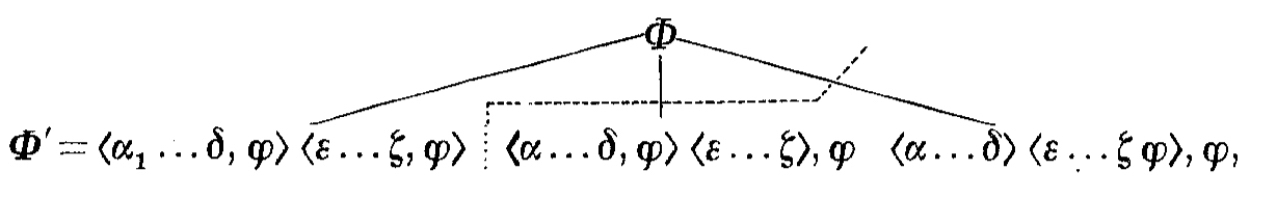
\includegraphics[width=350pt]{22prime}
}
but only the partial function on the left is possible, since the others belong to forbidden term systems (Pauli principle). It corresponds uniquely to the symmetry character
\nequ{23'}{
\left<1,\dots,i+1\right>\left<i+2,\dots,k+2\right>.
}
By permuting the cells $\alpha\dots\zeta$, $\varphi\varphi$ the other partial functions of the $A+B$ system are obtained. But now it is seen that the new partial functions is exactly the same as the system $A$, since the $\varphi$ occur in separate brackets, so they do not take part in the permutations $\overline{P}$ at all. The number of terms in (22') is then the same as those in (23), -- (23') is obviously partially degenerated.

Hence it is shown in general that no new splitting of the terms arises through interaction with closed shells\footnote{\?{Here Closed Shell is every paie of identical cells, not only degenerate cells}{Abgeschlossene Schale ist hier jedes Paar identischer Zellen, nicht etwa entarteter Zellen}. It is noted that our rule is not in contradiction with the spectroscopic \?{exchange rule}{Wechselsatz}, where the elements of the third row, which only differs from the alkali by two electrons of the $L_{II}$-shell, have a quadruplet system in addition to the doublet system. Thpugh the quadruplet belongs to different unperturbed occupations than the doublet corresponding to the alkalis.}. Here is probably the most visible property of a closed shell. It alone is to blame for the fact that there is a periodic system with homologous rows in which the elements show homologous spectroscopic and chemical properties.

Experiment has already long demanded "closed shells" with just this property \?{and we learned to fake it}{und zu fingieren gelehrt}; we learned to treat them as spherical charges\footnote{Cf Schr\"odinger's \WTF{Tauchbahnentheorie}, ZS. f. Phys. 4. 347, 1921; E. Fues, ZS. f. Phys. 11, 376, 1922.} etc, which betray little of the form those electrons, \WTF{wie es das Leuchtelektron ist}. Only the quantum mechanics supplies justification and understanding for this.

\section*{9. The term displacement.}
\subsection*{1.} We will go a step further and attempt to say something quantitative about the type of term displacements that arise through the possibilities for exchange with closed shells. In order to have a concrete case in view, we will explicitly specify the perturbation energies for examples I and II with the degeneration of \S7. Writing the 24 matrix elements (only 17 among them differ) and identifying two quantum cells $\alpha\equiv\beta$, the following matrix elements remain (the electron numbers are written as indices):
\nequ{24}{
\begin{array}{ll}
	E_0 = \int H\alpha_1^2 \alpha_2^2 \gamma_3^2 \delta_4^2 \D\tau & \\
	H_1 = \int H\alpha_1^2 \alpha_2^2 \gamma_3 \delta_3 \gamma_4 \delta_4 \D\tau &
	L = \int H\alpha_1\alpha_2\alpha_3\alpha_4\gamma_1\gamma_3\delta_2\delta_4\D\tau\\
	K_1 = \int H\alpha_1^2 \alpha_2 \gamma_2 \alpha_3\gamma_3\delta_4^2 \D\tau &
	M = \int H\alpha_1^2 \alpha_2 \alpha_3 \gamma_2 \delta_3 \gamma_4 \delta_4 \D\tau\\
	K_2 = \int H\alpha_1^2 a_2 \delta_2 \alpha_3 \delta_3 \gamma_4^2\D\tau
\end{array}
}

$E_0$ is the naive Coulomb interaction of the Schr\"odinger charges; $H_1,K_2,K_3$ correspond to the simple transpositions of class $(1\,2)$:
\uequ{
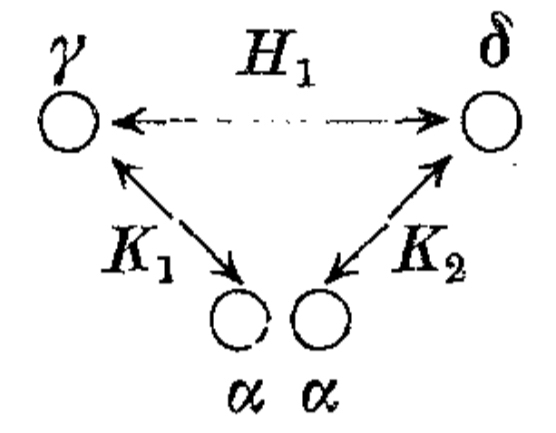
\includegraphics[width=100pt]{71}
}
while $L,M$ correspond to the higher permutation classes $(1\,2)(3\,4)$ and $(1\,2\,3)$. The matrix elements (24) arise from the general 4-body problem in the following manner, if the sums of all elements of the same classes are formed [cf (11)]:
\nequ{25}{
\begin{array}{ll}
	H_E & \to E_0\\
	H_{(1\,2)} & \to E_0 + H_1 + 2(K_1 + K_2)\\
	H_{(1\,2)(3\,4)} & \to H_1 + 2L\\
	H_{(1\,2\,3)} & \to 4M + 2(K_1 + K_2)\\
	H_{(1\,2\,3\,4)} & \to 4M + 2L
\end{array}
}
From the characters (13) and (14) follow the perturbation energies $E^1,E^2$.
\nequ{26}{
\begin{array}{cc}
	\Gamma_1 = \left[\left<1\,2\right>\left<3\,4\right>\right] &
	\Gamma_2 = \left<1\,2\,3\right>,4\\
	E^1 = E_0 + H_1 - (K_1 + K_2) + 2(L-M), &
	E^2 - H_1 - (K_1 + K_2) + 2M\\
\end{array}
}

\subsection*{2} If all cells $\alpha,\beta,\gamma$ are orthogonal\footnote{In many cases it will only be approximately so (cf loc cit). At any rate $L$ and $M$ will be small qith respect to the remaining matrix elements.}, then the only nonzero matrix elements are those corresponding to the simple transpositions $(1\,2)$, since the perturbation energy only contains $\frac{e^2}{\nu_{ik}}$ terms, so at most the coordinates of two electrons\footnote{Cf E. Schr\"odinger, Rapport to the fifth Solvay conference 1927 (at press).}. $L$ and $M$ vanish. Since in full generality the perturbation energy only contains simple transposition exchanges, the form of the various term systems with their exchange frequencies are much simplified. But at any rate it is to be noted that nevertheless the higher characters $\chi$ must also be calculated, since, as (25) shows, they go over into matrix elements of simple transpositions.

From (26) there still remain
\nequ{27}{
E^1 &= E_0 + H_1 - (K_1 + K_2)\\
E^2 &= E_0 - H_1 - (K_1 + K_2)
}
Interpreting the double cell $\alpha\alpha$ as the perturbing system $B$, the terms $-(K_1 + K_2)$ are the perturbation terms. They occur in both systems $\Gamma_1$ and $\Gamma_2$ with the same -- negative -- sign. If we imagine a \El{Li}-atom in the $\alpha\alpha\gamma$\footnote{$-K_1$ is apparently associated with the self-energy of the \El{Li}-atom, we understandably leave it for the future.}, a \El{H}-atom in $\delta$, then without the perturbation of the \El{Li}-$K$-shell one has
\uequ{
E^1 &= E_0 + H_1\\
E^2 &= E_0 - H_1,
}
which obviously corresponds exactly to formula (10) loc cit. $E^1$ would give a homopolar binding \El{LiH}, $E^2$ an elastic reflection. As is seen, the exchange possibilities of the \El{H}-electron with the \El{Li}-$K$-shell always acts with energy $-K_2$. From experiments with \El{H}-\El{H} it suspected that the sign of such matrix elements is negative, so $-K_2$ would be positive.

A dissociation energy for \El{LiH} of
\uequ{
-E^1 = -E_0 - H_1(+K_2)
}
is thereby decreased. I would suspect that here is one reason for the fact that the \El{LiH}, \El{Li${}_2$}, \El{Na${}_2$}, etc molecules have a much smaller dissociation energy than \El{H${}_2$}.

In general (22') shows that each partial function contains $\varphi$ in every antisymmetric bracket in each cell. In this manner $\varphi$ is amtisymmetrically connected with all other cells $\alpha\dots\delta$, $\varepsilon\dots\eta$. If (22') were completely degenerate, then it follows that all matrix elements $(\alpha\varphi)\dots(\eta\varphi)$ occur with negative signs, as in the example.

I would warmly thank Herrn Prof Schr\"odinger for his friendly interest with which he has always accompanied my papers, the International Education Board for the possibility of working with him.

Zurich, Physical Institute, October 1927.
\end{paper}